\Lecture{Jayalal Sarma}{Nov 11, 2020}{29}{Applying Cycle Index in Polya's Theorem}{Bhupathi Narasimha Rao}{$\alpha$}{JS}
\section{Recall the definitions of Type and Cycle Index Polynomial}
Let $G$ be the set of some permutations of $\Omega$ , every $g \in G$ can be decomposed into a collection of disjoint cycles .\\
\textbf{Example 1:-} Consider $g=\{2,3,1,5,4\}$ which is a permutation on set $\{1,2,3,4,5\}$ . So , the permutation $g$ can be written as $(1~2~3)(4~5)$ .\\
\textbf{Example 2:-} Identity on set $[n]$ can be written as $g=(1)(2)(3)\dots(n)$ which is $n$-cycles of length $1$.\\\\
\textbf{Type of a permutation :-} A permutation $\pi$ is said to be of type $(b_1,b_2,\dots,b_m)$ if 
$$b_i = \textrm{\# of $i$-length cycles in the cyclic representation of $\pi$}$$
\textbf{Example 1:-} Type of an identity permutation is $(n,0,\dots,0)$ .\\
\textbf{Example 2:-} Type of the permutation $g=(1~2~3)(4~5)$ is $(0,1,1,0,0)$ .\\\\
\textbf{Cycle index Polynomial :-}As discussed in previous lectures , a monomial is associated corresponding to every type as follows :
$$(b_1,b_2,\dots,b_m)\longleftrightarrow x_1^{b_1}x_2^{b_2}\dots x_m^{b_m}$$
And the cycle index polynomial of $G$ is defined as:
$$P_G(x_1,x_2,\dots,x_n)=\frac{1}{|G|}\sum_{g\in G}(x_1^{b_1}x_2^{b_2}\dots x_n^{b_n})~~~\textrm{where $(b_1,b_1,\dots,b_n)$ is the type of $g$}$$
\textbf{Example 1:-} Let $G=\{e,(1~2),(3~4),(1~2)(3~4)\}\leq S_4$ , then 
$$P_G(x_1,x_2,x_3,x_4) = \frac{1}{4}\left(x_1^{4}+x_1^{2}x_2+x_1^{2}x_2+x_2^{2}\right)$$
\textbf{Example 2:-} Let $G=\{e,(1~2),(1~3),(2~3),(1~2~3),(1~3~2)\}=S_3$ , then 
$$P_G(x_1,x_2,x_3) = \frac{1}{6}\left(x_1^{3}+x_{1}x_{2}+x_{1}x_{2}+x_{1}x_{2}+x_3+x_3\right)=\frac{1}{6}\left(x_1^{3}+3x_{1}x_{2}+2x_3\right)$$
\textbf{Why are we doing this :} The connection to Polya's Theorem will be found by the end of this lecture .
\section{Polya's Theorem (Simpler version)}
\begin{theorem}Let $G$ be the group of symmetry acting on $\Omega$ (set of different coloring of the underlying object) , then 
$$\textrm{\# of distinct color patterns with $k$-colrs } = P_G(k,k,\dots,k)$$
\begin{proof}
Let the Domain be of size $m$ and we have $k$ colors , then  $|\Omega|=k^m$ . Using Burnsides's Lemma ,  
\begin{align*}
    \textrm{\# of distinct colorings} &= \textrm{\# of different orbits of G acting on} \Omega\\
    &= \frac{1}{|G|}\sum_{g\in G} |fix(G)|
\end{align*}
We have to compute $|fix(g)|$ for $g\in G$ . For example , the cyclic structure of $g$ be $(1~2)(3~4)$ , the coloring should be such that the domain under the permutation looks the same . So , the corners $1,2$ should have same color and $3,4$ should have same color . So , total number of colorings such that the domain looks the same under the permutation $g = k^2$ . Hence all the corners in one cycle should get the same color . So , consider the type of some permutation $g=(b_1,b_2,\dots,b_m)$ , then
\begin{align*}
    &\textrm{$b_1$ cycle of length $1$ can have $k^{b_1}$ possible coloring}\\
    &\textrm{$b_2$ cycle of length $2$ can have $k^{b_2}$ possible coloring}\\
    &\dots\\
    &\dots\\
    &\textrm{$b_m$ cycle of length $m$ can have $k^{b_m}$ possible coloring}
\end{align*}
Therefore , \# of colors fixed by $g=|fix(g)|=k_{b_1}*k^{b_2}*\dots*k^{b_m} = x_1^{b_1}*x_2^{b_2}*\dots*x_m^{b_m} ~~~\\\textrm{where } x_i=k~\forall i\in [k]$

Hence , \# of distinct color patterns with $k$-colors is 
$$\frac{1}{|G|}\sum_{g\in G}\left(k^{b_1}*k^{b_2}*\dots*k^{b_m}\right)= P_G(k,k,\dots,k)$$
\end{proof}
\end{theorem}
\section{Examples}
\textbf{Example 1:-} Coloring necklace with 3 regular beads with black and white colors . Symmetries are rotation with respect to the axis passing through the center and rotation with respect to the axis passing through one vertex and center of the opposite edge . Hence ,   $$G=\{e,R_{120},R_{240},F_{12},F_{23},F_{31}\}$$ and cyclic representations are $\{(1)(2)(3),(1~2~3),(1~3~2),(1~2),(2~3),(3~1)\}=S_3$ . Cyclic index polynomial corresponding to $G$ is:
$$P_G(x_1,x_2,x_3) = \frac{1}{6}\left(x_1^3+3x_1x_2+2x_3\right)$$
Hence \# of different colorings with $2$ colors $=\frac{1}{6}\left(2^3+3*2^2+2*2\right) = 4$\\
\textbf{Example 2:-} Consider cube coloring on faces and the symmetries group $G$ defined previously as :


\begin{tabular}{|l|l|}
    \hline
\thead{\textbf{Permutation}} & \thead{\textbf{Corresponding Monomial}} \\\hline
Identity $(e)$ & $x_1^6$\\
$180^0$ rotation wrt axis through centers of opposite faces ($3$ of them) &  $3x_1^{2}x_2^{2}$\\
$180^0$ rotation wrt axis through centers of opposite edges ($6$ of them) &  $6x_2^3$\\
$90^0$ rotation wrt axis through centers of opposite faces ($3$ of them) &  $3x_1^2x_4$\\
 $270^0$ rotation wrt axis through centers of opposite faces ($3$ of them) & $3x_1^2x_4$\\
 $120^0$ rotation wrt axis thorough center and opposite corners ($4$ of them) & $4x_3^2$ \\
 $240^0$ rotation wrt axis through center and opposite corners ($4$ of them)  &  $4x_3^2$\\ \hline
    \end{tabular}
    
    
Hence cyclic index polynomial corresponding to above symmetries is:
$$P_G(x_1,x_2,x_3,x_4,x_5,x_6)=\frac{1}{24}\left(x_1^6+3x_1^2x_2^2+6x_2^3+3x_1^2x_4+3x_1^2x_4+4x_3^2+4x_3^2\right)$$
$$\implies P_G(x_1,x_2,x_3,x_4,x_5,x_6)=\frac{1}{24}\left(x_1^6+6x_1^2x_4+3x_1^2x_2^2+8x_3^2+6x_2^3\right)$$
\textit{Question:-} If the coloring is done on the corners rather than faces with same $G$, does the polynomial change ?
\\
\textbf{Example 3:-} Square Problem discussed in previous lectures , $$G=\{e,R_{90},R_{180},R_{270},H,V,D,D^{\prime}\}$$ and corresponding cyclic representations are $$\{(1)(2)(3)(4),(1~2~3~4),(1~3)(2~4),(1~4~3~2),(1~4)(2~3),(1~2)(3~4),(1~3),(2~4)\} {\ensuremath <} S_4$$
There is some connection between $(1~2~3~4)$ and $(1~3)(2~4)$ . If the permutation $(1~2~3~4)$ is applied twice to the domain (square) , we get the permutation $(1~3)(2~4)$ . That is $(1~2~3~4)$ composed with itself gives $(1~3)(2~4)$ . $(1~3)(2~4)$ composed with $(1~2~3~4)$ gives $(1~4~3~2)$ .

Hence the set $\{e,R_{90},R_{180},R_{270}\}$ forms a subgroup . Suppose the permutation $(1~2~3~4)$ be $g$ , then corresponding permutations are $\{e,g,g^2,g^3\}$ ($g^4$ is an identity) \\

Suppose we have a group of symmetry as (considering $n$ to be even): $$G=\{e,g,g^2,g^3,\dots,g^k\}=\{e,(1~2~3\dots~n),(1~3~5~\dots~n-1)(2~4~4~\dots~n),\dots\dots\}~~~\textrm{with $g^{k+1}$ as identity}$$
Groups of type $G$ are called as cyclic groups . The monomials corresponding to each permutations are as follows:\\
\begin{tabular}{|l|l|}
    \hline
\thead{\textbf{Permutation}} & \thead{\textbf{Corresponding Monomial}} \\\hline
$e$ & $x_1^n$\\
$g$ & $x_n$\\
$g^2$ & $x_{\frac{n}{2}}^2$\\
$g^3$ & $x_{\frac{n}{4}}^4$\\
\dots & \dots\\ \hline
    \end{tabular}\\
So , the cyclic index polynomial corresponding to $G$ can be written as:
$$P_G(x_1,x_2,\dots,x_n)=\frac{1}{n}\sum_{d\mid n}\phi(\frac{n}{d})x_{\frac{n}{d}}^d$$
where $\phi(.)$ is the Euler's function . $\phi(n)$ = \# of positive integers up to $n$ that are relatively prime to $n$ . If $n$ is odd ,
$$P_G(x_1,x_2,\dots,x_n) = \frac{1}{2n}\sum_{d\mid n}x_{\frac{n}{d}}^d + \frac{1}{2}x_1x_2^{\frac{n-1}{2}}$$
\section{Dihedral Group}
For the permutations $\sigma=(1~2~\dots~n)$ and $\pi=(2~n)(3~n-1)$ , the group defined as:
$$D_n = \{e,\sigma,\sigma^2,\dots,\sigma^{n-1},\pi\sigma,\pi\sigma^2,\dots,\pi\sigma^{n-1}\}$$
are called Dihedral groups . Here $D_n$ is a Dihedral group .\\ 
\textbf{Example 1:-}
Consider permutation on a square $\sigma = (1~2~3~4)$ and $\pi=(2~4)(3~3)=(2~4)(3)(1)$ , then 
\begin{align*}
    \pi\sigma &= (2~4)(3)(1)(1~2~3~4)\\
    &= (2~1)(3~4)\\
    &= V
\end{align*}
\textbf{Observation:-}$|D_3|=6=|S_3|$ and $|D_4|=8\le|S_4|$

\section{Polya's Theorem (General Version)}
\textbf{Motivating Question:- }How many in-equivalent colorings are there using $3$ black and $1$ white ? 
\begin{figure}[h!]
    \centering
    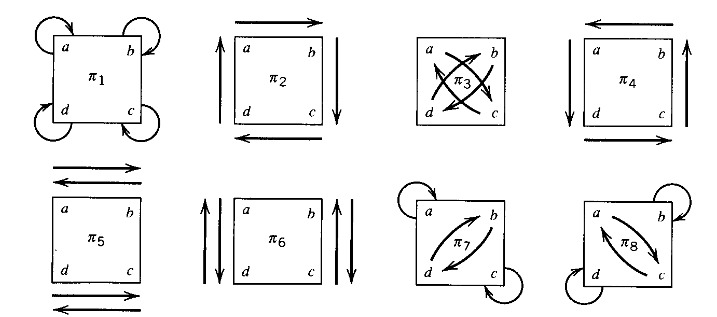
\includegraphics[width=0.6\linewidth]{images/Set-G.jpeg}
    \caption{Symmetries on square}
\end{figure}
\begin{figure}[h!]
    \centering
    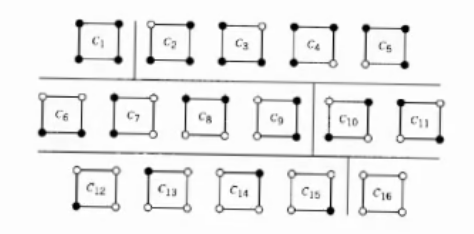
\includegraphics[width=0.6\linewidth]{images/Square-colorings-black-white.png}
    \caption{All possible coloring on square with black and white}
\end{figure}

\textbf{AIM :-} To write a polynomial $Q(b,w)$ such that coefficient of $b^2w^2=$ \# of inequivalent colorings with $2$ Black and $2$ White colors . Similarly , coefficient fo $b^3w=$\# of inequivalent colorings with $3$ Black and $1$ White colors .

\qquad Consider the identity permutation $e$ , no.of colorings fixed by $e$ considering $2$ colors = $16$ . And no.of colorings fixed by $e$ considering $3$ Black and $1$ White = $4$ (from the above fig.)
If we write this down for the permutations fixed by $e$ , the expression will be as :
$$b^4+4b^3w+4bw^3+6b^2w^2+w^4=(b+w)^4$$
Let us classify elements of $\Omega=\{C_1,C_2,\dots,C_{16}\}$ into their corresponding coloring structures . The classification will be as follows :
\begin{align*}
    b^4 &\longleftrightarrow T_1=\{C_1\}\\
    b^3w &\longleftrightarrow T_2=\{C_2,C_3,C_4,C_5\}\\
    b^2w^2 &\longleftrightarrow T_3=\{C_6,C_7,C_8,C_9,C_{10},C_{11}\}\\
    bw^3 &\longleftrightarrow T_4=\{C_{12},C_{13},C_{14},C_{15}\}\\
    w^4 &\longleftrightarrow T_5=\{C_{16}\}
\end{align*}
Suppose we want to know how many inequivalent colorings are possible with $3$ Black and $1$ White on a square when group $G$ is applied , then it is enough to apply the group $G$ on $T_2$ and count the inequivalent colorings . So , now we need to understand how many inequivalent colorings are there in each $T_i$ .

\qquad $G$ acting on $T_i$ is well-defined . It is because when a rotation/flip is applied on a square , the number of colors or number of vertices is not changed . The image will be one of the elements of $T_i$ itself . Hence , it is well-defined . So , for finding number of inequivalent colorings of a specific structure (like $3$ Black and $1$ White) , it is enough to apply $G$ on corresponding $T_i$ ($T_2$ if $3$ Black and $1$ White) and apply Burnside's lemma (\textit{i.e.,} compute $|fix(g)| \forall g\in G$) .\\\\
\textbf{Example 1:-} Find the number of inequivalent colorings using $3$ Black and $1$ White when $G=\{e,R_{90},R_{180},R_{270},H,V,D,D^{\prime}\}$ applied on $\Omega$ . \\
\textbf{Solution :-} Consider action of $G$ on $T_2=\{C_2,C_3,C_4,C_5\}$ , 
\begin{align*}
    \textrm{\# of inequivalent colorings }&= \frac{1}{|G|}\sum_{g\in G}|fix(g)|\\
    &= \frac{1}{8}\left(|fix(e)|+|fix(D)|+|fix(D^{\prime})|\right)~~~\textrm{Action of other $g$'s gives $|fix(g)|=0$}\\
    &= \frac{1}{8}\left(4+2+2\right)\\
    &= 1
\end{align*}\\
\textbf{Example 2:-} Find the number of inequivalent colorings using $2$ Black and $2$ White when $G=\{e,R_{90},R_{180},R_{270},H,V,D,D^{\prime}\}$ applied on $\Omega$ . \\
\textbf{Solution :-} Consider action of $G$ on $T_3=\{C_6,C_7,C_8,C_9,C_{10},C_{11}\}$ , 
\begin{align*}
    \textrm{\# of inequivalent colorings }&= \frac{1}{|G|}\sum_{g\in G}|fix(g)|\\
    &= \frac{1}{8}\left(|fix(e)|+|fix(R_{180})|+|fix(H)|+|fix(V)|+|fix(D)|+|fix(D^{\prime})|\right)\\
    &= \frac{1}{8}\left(6+2+2+2+2+2\right)\\
    &= 2
\end{align*}\\
\textbf{Example 3:-} Given a permutation $g$ with cycle structure $(1~2)(3)(4)$ . How many inequivalent colorings are possible with different combinations of Black and White colors ?\\
\textbf{Solution :-} We have to count number of colorings that are fixed by $g$ . So , $1,2$ should have same color , $3,4$ can have any color . Hence , the expression $(b^2+w^2)(b+w)(b+w)$ represents the possible colorings where coefficient of each term correspond to the number of colorings which are inequivalent with that color structure . 
$$(b^2+w^2)(b+w)(b+w) = b^4+2b^3w+2b^2w^2+2bw^3+w^4$$
Hence , $g$ fixes square with $4$ corners coloured Black , $4$ corners colored White , $2$ squares colored with $3$ Black and $1$ White , $2$ squares colored with $2$ Black and $2$ White , $2$ squares colored with $1$ Black and $3$ White .\\
\textbf{Example 4:-} Given permutation $g$ with cycle structure $(1~2)(3)(4)(5~6~7)$ , the colorings which are fixed by $g$ is given by $(b^2+w^2)(b+w)(b+w)(b^3+w^3)$ .\\
\section{Polya's Theorem}
\begin{theorem}
If the colors $\alpha_1,\alpha_2,\dots,\alpha_k$ are used , then 
$$\textrm{\# of inequivalent colorings expressed as generating function } = P_G(\sum_{i=1}^{k}\alpha_i,\sum_{i=1}^{k}\alpha_i^2,\dots)$$
\end{theorem}\\
\textbf{Example 1:-} Consider the necklace with $3$-half beads colored with Black and White . The group of symmetry is $G=\{e,R_{120},R_{240}\}$ . Then generating function is :
$$P_G(x_1,x_2,x_3) &= \frac{1}{3}\left(x_1^3+2x_3\right)$$
Substitute $x_1$ with $(b+w)$ , $x_2$ with $(b^2+w^2)$ and $x_3$ with $(b^3+w^3)$ . Then the generating function using Polya's theorem is:
\begin{align*}
    P_G(b+w,B62+w^2,b^3+w^3) &= \frac{1}{3}\left((b+w)^3+2(b^3+w^3)\right)\\
    &= b^3+w^3+b^2w+bw^2
\end{align*}

\Lecture{Jayalal Sarma}{Nov 12, 2020}{30}{Partial Order}{Prasannasai Babu}{$\alpha$}{JS}
\section{Formal Definition and Examples}
A partial order is a homogeneous binary relation $\leq$ over a set $X$ satisfying particular axioms which are discussed below. When $x\leq y$, we say that $x$ is related to $y$. (This does not imply that $y$ is also related to $x$, because the relation need not be symmetric.)\\\\
The axioms for a partial order state that the relation $\leq$ is reflexive, antisymmetric, and transitive. That is, $\forall a, b, c \in X$, it must satisfy:\\\\
\textbf{Reflexivity:} $a\leq a$\\
\textbf{Transitivity:} if $a\leq b \And b \leq c$ then $a \leq c$\\
\textbf{Antisymmetry:} if $a \leq b \And b \leq c$ then $a = b$\\\\
Partial Ordered set is also called as \textbf{"Poset"}\\\\
\textbf{Example 1:} Natural numbers $\mathbb{N}$ with $\leq$ order\\
\textbf{Example 2:} Natural numbers $\mathbb{N}$ with $|~$(division) relation, That is $a\leq b$ if $a | b$\\
\textbf{Example 3:} Set $X = \{1,2,4,3,7,6,9,10\}$ with $|$ relation. In this example $1$ is less than or equal to every other element in the set as $1$ divides every other element in the set. Now take two elements $3$ and $7$, now we can't say $3 \leq 7 \And 7 \leq 3$ as $3$ doesn't divide $7$ and $7$ doesn't divide $3$. So elements $3$ and $7$ are incomparable.\\
This leads to the notion of comparable and incomparable elements.\\
\textbf{Example 4:} Polynomials over $|~$ (division) relation.\\
\textbf{Example 5:} Words(over English alphabets) over lexicographic order or dictionary order or graded lexicographic order.\\\\
A partial order is said to be total order of there are no incomparable elements.\\\\
\textbf{Example 6:} Set of subsets of $[n]$ and the ordering is by inclusion. This is not a total order.\\
\textbf{Example 7:} Set of the strings over the alphabet $\{0,1\}$ of length $n$ over the ordering for two strings $x,y$ we say $x\leq y$ if $\forall i \in [n],~x_i \leq y_i$\\\\
We know that there is a bijection between the sets in Example $6$ and Example $7$, and it turns out that the bijection is not only a bijection and it also preserves the ordering. Our claim here is 
for $A,B \subseteq [N]$, $A \subseteq B \iff \phi(A) \leq \phi(B)$, where $\phi$ is the bijective function.
\section{Representation of Posets}
A poset $p = (X,\leq)$ can naturally representes as a directed graph with $X$ as the vertex set and the directed edges $xy$ if $x$ and $y$ have a relation $x \leq y$. For example take three elements $a, b, c$ from $X$, now we will draw edge from $a$ to $b$ if $a\leq b$ and edge from $b$ to $c$ if $b \leq c$, Now we don't need to draw edge from $a$ to $c$, although we know $a \leq c$ through transitivity, because it unnecessarily increases the size of the graph.\\
Graph $G$ has vertices V as $V = X$ and edges E as $E = \{(x,y) | x,y \in X, x \leq y \}$\\
The graphs that represents these posets are called as \textbf{Hasse diagram}. So transitive closure of the graph $G$ is the graph of the relation.
\section{New terms and Notations}
\textbf{Chain:} $C \subseteq X$ is said to be a chain if every pair of elements in $C$ is comparable. The chain C is a total order.\\\\
\textbf{Height of Poset:} Length of the longest chain.\\\\
\textbf{Anti-Chain:} $A \subseteq X$ is said to be anti-chain if every pair of elements in $A$ is incomparable.\\\\
\textbf{Width of Poset:} Size of largest Anti-Chain.\\\\
\textbf{Maximal Elements:}  $\{x \in X | \forall y \in X, y \leq x ~or~ x || y$\}. Here the symbol $||$ represents incomparability.\\\\
\textbf{Minimal Elements:} $\{x \in X | \forall y \in X, x \leq y ~or~ x || y\}$. Here the symbol $||$ represents incomparability.\\\\
\textbf{Note:} Maximal elements set and Minimal elements set, both are anti-chains.
\section{Theorems on partitioning poset into chains and anti-chains}
\begin{theorem}
Every poset $P(X,\leq)$ can be partitioned into height($P$) many antichains(and not less).
\begin{proof}
We know that every element in anti-chain are incomparable. Now take the set of the elements in the longest chain. The length of the chain is height($P$). We know every element in the chain are comparable. So every element in the longest chain must belong to different anti-chain. So there must be atleast height($P$) many anti-chains.
\\\\
Now, let's look at alternate proof using induction.\\\\
\textbf{Claim:} For any max chain $C$ of poset $P$, min($P$) $\cap ~ C ~\neq~ \phi$\\
We will do induction on height($P$). Now consider the longest chain C and remove min($P$) from $P$ to get $P^'$, so height of $P^'$ is height($P$) $ - 1$. We assume that the theorem is true for $P^'$.\\
Applying induction hypothesis,\\
Now add min($P$) to $P^'$, the height will be increased by $1$ that is height($P$) $=$ height($P^'$) $+ 1$ and adding min(P) will result in increasing number of anti-chains by $1$ to get full partition of $P$.
\end{proof}
\end{theorem}
\begin{theorem}
\textbf{Dilworth's Theorem:} Every poset $P(X,\leq)$ can be partitioned into width($P$) many chains(and no less).
\begin{proof}
We will prove this by applying induction on the size of set $X$ i.e., $|X|$
Let's take the width of the poset as $w$. Let $A \subseteq X$ be the anti-chain with size $w$. Now we will decompose $P$ into $P_1 = (X_1,\leq)$ and $P_2 = (X_2,\leq)$.
$$X_1 = \{y \in X | \exists~ x ~ \in ~ A, x \leq y\}$$
$$X_2 = \{y \in X | \exists~ x ~ \in ~ A, y \leq x\}$$
\textbf{Claim:} $X_1 \cap X_2 = A$. So $A \subseteq X_1 \cap X_2$.\\
Suppose $y \in X_1 \cap X_2$, then $\exists~ x_1, x_2$ such that $x_1 \leq y \leq x_2$.\\
Now $x_1$ becomes comparable to $x_2$. But $x_1, x_2 \in A$ which is anti-chain.\\
$\Rightarrow x_1 = x_2 = y$\\
$\Rightarrow y \in A$\\
Suppose $|X_1| < |X| \And |X_2| < |X|$
We can apply induction hypothesis on $P_1$ and $P_2$ to get chains $C_1, C_2, C_3, \ldots C_w$ and ${C^'}_1, {C^'}_2, {C^'}_3, \ldots {C^'}_w$ each of length $w$.\\
We know,\\
$$A = min(P_1) = max(P_2)$$
We can join the corresponding chains to get chains of poset $P$. Let the elements of set $A = \{a_1,a_2,a_3,\ldots,a_w\}$.\\
Without loss of generality, let's assume that $C_1$ ends at $a_1$, $C_2$ ends at $a_2$ and so on upto $C_w$ ends at $a_w$. Similarly $C_1^'$ starts as $a_1$, $C_2^'$ starts at $a_2$ and so on upto $C_w^'$ starts at $a_w$. Now partition of $X$ for $P$ can be $C_1 \cdot {C_1^'}, ~C_2 \cdot {C_2^'}$ and so on upto $C_w \cdot {C_w^'}$.\\\\
We need to handle the case when $|X_1| = |X|$ or $|X_2| = |X|$.\\
If $|X_1| = |X|$ that means $X_1 = X$, which in turn means $A = min(P)$. Similarly if we choose $A = max(P)$ then $X_2 = X$ and $|X_2| = |X|$. If there are anti-chains of size $w$ which are not min($P$) and max($P$), then we can do the same like above.\\\\
But if it is the case that the only max sized anti-chains are max($P$) or min($P$) or both, we should look for alternate approach.\\\\
Now consider any max chain in P, and remove that chain $C$ from $P$ to get $P^'$. So now,\\
$$max(P) \cap C \neq \phi \And min(P) \cap C \neq \phi$$
We can apply induction hypothesis to get a decomposition of $P^'$ in less than $w$ many chains. Now put the $C$ back to get decomposition into $w$ many chains which partition $X$.

\end{proof}
\end{theorem}

\section{Applications of partial order}
\textbf{Application 1:} Proof of Erdős–Szekeres theorem\\
\begin{theorem}
Every sequence of $rs+1$ distinct integers, there must exist an increasing sequence of length $r+1$ or decreasing sequence of length $s+1$.
\begin{proof}
Let $a_1,a_2,a_3,\ldots,a_n$ be the sequence of length $n$ where $n = rs+1$.\\
Define ordering of the sequence as $a_i \leq a_j$ if $i\leq j$ and $a_i \leq a_j$. It is transitive, reflexive and anti-symmetric. So it is a partial order. So we define chains and anti-chains in this poset. A chain in this poset means the elements are in the increasing order.\\
$\Rightarrow$ A chain in this poset $\rightarrow$ increasing sub-sequence.\\
Similarly an anti-chain in this poset means the elements are in the decreasing order.\\
$\Rightarrow$ An anti-chain in this poset $\rightarrow$ decreasing sub-sequence.\\
Suppose there is no anti-chain(decreasing sub-sequence) of size $s+1$.
$$\Rightarrow w(P) \leq s$$
By Dilworth's theorem there is a decomposition of $P$ into atmost $s$ many chains. So there exists at least one chain with $r+1$ elements, otherwise there will be only $r\times s$ elements in the ground set. But we have $rs+1$ elements. Therefore there must exist a chain with $r+1$ elements which is an increasing sub-sequence.
\end{proof}
\end{theorem}
.\\
\textbf{Example for size of chain and anti-chain}\\
We know there is a bijection between example $6$ and example $7$ in section $30.1$ i.e., between the sets\\
$\Rightarrow$ subset poset of subsets of [n] $\rightarrow$ Boolean strings poset of length $n$.\\
The max length of the chain is $n+1$. Intutively we can say that maximum size of the anti-chain is $n \choose \frac{n}{2}$. Let's look how to prove it in the next lecture by Sperner's theorem.
\Lecture{Jayalal Sarma}{Nov 13, 2020}{31}{Sperner's Theorem}{Prasannasai Babu}{$\alpha$}{JS}
\section{{Sperner's theorem}}
\begin{theorem}
\textbf The maximum size of any anti-chain in the subset poset(Example $6$ of $30.1$) is $n \choose \frac{n}{2}$.
\begin{proof}
The subset poset is equivalent to boolean strings of length $n$ poset. Now let's represent boolean string poset as $B_n$. We need to prove width($B_n$) = $n \choose \frac{n}{2}$.\\
Let us first show that width($B_n$) is atleast $n \choose \frac{n}{2}$. We can show one anti-chain of size $n \choose \frac{n}{2}$, that is subsets of size $\frac{n}{2}.$\\
Now we need to show that any anti-chain in $B_n$ must have size $\leq ~{n \choose \frac{n}{2}}$\\\\
Let F be any anti-chain in $B_n$. We need to show $|F| \leq {n \choose \frac{n}{2}}$. Let us say,\\\\
A permutation $\pi \in S_n$ is said to meet $A \subseteq \{1,2,\ldots,n\}$ if $A$ forms prefix of $\pi$. This statement meaning is, Let's say $|A| = k$ then $\pi$ said to meet $A$ if $A = \{\pi(1),\pi(2),\ldots,\pi(k)\}$.\\\\

Consider each subset in $F$ and consider permutations meeting them, As we are taking subsets from $F$, they are incomparable. Hence a single permutation can't meet both $A$ and $B$.Now let's count the size of
$$\sum_{A\in F} \bigg|\{\pi | \pi ~meets~ A\}\bigg|$$
As single permutation can meet only one subset of F,
$$\sum_{A\in F} \bigg|\{\pi | \pi ~meets~ A\}\bigg| \leq n!$$
Now number of permutations that can meet set $A$ of size $k$ is $k! \times (n-k)!$.So,
$$\sum_{A\in F} |A|! \times (n-|A|)! ~~~\leq~~~ n!$$
Bring that RHS term to LHS, now 
$$\sum_{A\in F} \frac{1}{\frac{n!}{|A|! \times (n-|A|)!}} ~~~\leq~~~ 1$$
$$\sum_{A\in F} \frac{1}{{n \choose {|A|}}} ~~~ \leq ~~~ 1$$
We can substitute $n \choose \frac{n}{2}$ in place of $|A|$ and the inequality still holds.
$$\sum_{A\in F} \frac{1}{{n \choose \frac{n}{2}}} ~~~ \leq ~~~ 1$$
$$\sum_{A\in F} 1  ~~~ \leq ~~~ {n \choose \frac{n}{2}}$$
$$|F| ~~~\leq~~~ {n \choose \frac{n}{2}}$$
We showed that,
$$|F| ~~~\leq~~~ {n \choose \frac{n}{2}} \And |F| ~~~\geq~~~ {n \choose \frac{n}{2}}$$
Hence the max size of the anti-chain $F$ is 
$$|F| ~~~=~~~ {n \choose \frac{n}{2}} $$
Hence proved.
\end{proof}
\end{theorem}




